\part{Celestial Sphere \&  Asymptotic Flat Spacetime}
% 计数器清零,每个part都要引用,除了part1
\setcounter{theorem}{0}
\setcounter{definition}{0}
\setcounter{lemma}{0}
\setcounter{sidenote}{1}

\section{Carter-Penrose diagram}
Minkowski时空的度规在球坐标系下可以写为:

\begin{equation}
	ds^2=-dt^2+dr^2+r^2\eqnmarkbox[red]{node}{\left(d\theta^2+\sin^2\theta d\phi^2\right)}
\end{equation}
\annotate[yshift=0.7em]{}{node}{$d{\Omega_2}^2$}
定义retarded和advanced坐标为:
\begin{equation}
	u\equiv t-r,\quad v\equiv t+r
\end{equation}
这个坐标系下度规重写为:
\begin{equation}
	ds^2=-dudv+\frac{(u-v)^2}{4}d{\Omega_2}^2,\quad -\infty<u\leq v <+\infty
\end{equation}
由于时空具有球对称性,所以考虑忽视角向,只考虑径向,那么时空图$t\mbox{-}r$上每一个点代表一个球面,径向光线意味着$u$或$v$是常数。时空的无限远有不同的趋向方式,这也导致了不同的无穷远定义:
\begin{marginfigure}
\begin{center}
	\tikzset{every picture/.style={line width=0.75pt}} %set default line width to 0.75pt        
	
	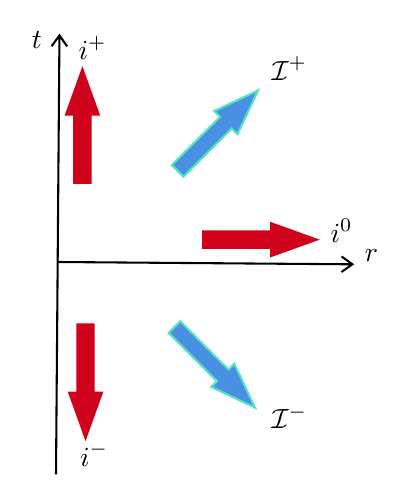
\begin{tikzpicture}[x=0.75pt,y=0.75pt,yscale=-0.75,xscale=0.75]
		%uncomment if require: \path (0,609); %set diagram left start at 0, and has height of 609
		
		%Shape: Axis 2D [id:dp7821872331367214] 
		\draw  (196.6,214.86) -- (385.94,216.34)(197.75,69.29) -- (195.53,351.32) (378.98,211.29) -- (385.94,216.34) -- (378.9,221.29) (192.69,76.25) -- (197.75,69.29) -- (202.69,76.33)  ;
		%Up Arrow [id:dp5623641448201375] 
		\draw  [color={rgb, 255:red, 208; green, 2; blue, 27 }  ,draw opacity=1 ][fill={rgb, 255:red, 208; green, 2; blue, 27 }  ,fill opacity=1 ] (202,120.2) -- (212.5,91) -- (223,120.2) -- (217.75,120.2) -- (217.75,164) -- (207.25,164) -- (207.25,120.2) -- cycle ;
		%Up Arrow [id:dp9355069637780506] 
		\draw  [color={rgb, 255:red, 208; green, 2; blue, 27 }  ,draw opacity=1 ][fill={rgb, 255:red, 208; green, 2; blue, 27 }  ,fill opacity=1 ] (225,298.8) -- (214.5,328) -- (204,298.8) -- (209.25,298.8) -- (209.25,255) -- (219.75,255) -- (219.75,298.8) -- cycle ;
		%Up Arrow [id:dp8020921103254861] 
		\draw  [color={rgb, 255:red, 208; green, 2; blue, 27 }  ,draw opacity=1 ][fill={rgb, 255:red, 208; green, 2; blue, 27 }  ,fill opacity=1 ] (333.8,190) -- (363,200.5) -- (333.8,211) -- (333.8,205.75) -- (290,205.75) -- (290,195.25) -- (333.8,195.25) -- cycle ;
		%Up Arrow [id:dp5136238103533108] 
		\draw  [color={rgb, 255:red, 80; green, 227; blue, 194 }  ,draw opacity=1 ][fill={rgb, 255:red, 74; green, 144; blue, 226 }  ,fill opacity=1 ] (297.24,117.91) -- (325.31,104.69) -- (312.09,132.76) -- (308.37,129.05) -- (277.4,160.02) -- (269.98,152.6) -- (300.95,121.63) -- cycle ;
		%Up Arrow [id:dp5383249274435937] 
		\draw  [color={rgb, 255:red, 80; green, 227; blue, 194 }  ,draw opacity=1 ][fill={rgb, 255:red, 74; green, 144; blue, 226 }  ,fill opacity=1 ] (310.09,280.24) -- (323.31,308.31) -- (295.24,295.09) -- (298.95,291.37) -- (267.98,260.4) -- (275.4,252.98) -- (306.37,283.95) -- cycle ;
		
		% Text Node
		\draw (332,81) node [anchor=north west][inner sep=0.75pt]   [align=left] {$\displaystyle \mathcal{I}^{+}$};
		% Text Node
		\draw (332,305) node [anchor=north west][inner sep=0.75pt]   [align=left] {$\displaystyle \mathcal{I}^{-}$};
		% Text Node
		\draw (208,68) node [anchor=north west][inner sep=0.75pt]   [align=left] {$\displaystyle i^{+}$};
		% Text Node
		\draw (209,329) node [anchor=north west][inner sep=0.75pt]   [align=left] {$\displaystyle i^{-}$};
		% Text Node
		\draw (178,65) node [anchor=north west][inner sep=0.75pt]   [align=left] {$\displaystyle t$};
		% Text Node
		\draw (370,185) node [anchor=north west][inner sep=0.75pt]   [align=left] {$\displaystyle i^{0}$};
		% Text Node
		\draw (392,205) node [anchor=north west][inner sep=0.75pt]   [align=left] {$\displaystyle r$};
	\end{tikzpicture}
\end{center}
\caption{共形无穷远定义}
\end{marginfigure}
\begin{itemize}
	\item[$i^+$]:类时未来无穷远,$r$一定,$t\to+\infty$;
	\item[$i^-$]:类时过去无穷远,$r$一定,$t\to-\infty$;
	\item[$i^0$]:类空无穷远,$t$一定,$r\to+\infty$;
	\item[$\mathcal{I}^+$]:类光未来无穷远,$u$一定,$r\to+\infty$;
	\item[$\mathcal{I}^-$]:类光过去无穷远,$v$一定,$r\to+\infty$;
\end{itemize}
这五个无穷远合称为\textbf{共形无穷远}。

但是无穷远还是一个靠想象的概念,无法在这样的图中表现出来,继续考虑坐标变换,变到所谓光锥坐标:
\begin{equation}
	U\equiv\arctan u ,\quad V\equiv\arctan v
\end{equation}
度规在光锥坐标下变为:
\begin{equation}
	ds^2=\frac{1}{4\cos^2U\cos^2V}\cdot\left(-4dUdV+\sin^2(V-U)d{\Omega_2}^2\right),\quad -\frac{\pi}{2}<U\leq V<\frac{\pi}{2}
\end{equation}
现在我们牺牲对距离的精确描述,考虑Weyl变换之后,丢掉共形因子后的度规:
\begin{equation}\label{eq:15.6}
	\tilde{ds}^2=-4dUdV+\sin^2(V-U)d{\Omega_2}^2
\end{equation}
这样消去了在$\pm\frac{\pi}{2}$处的坐标奇性,我们称之为\textbf{共形紧化}。可以证明\cite{blau},两个相差共形变换的度规具有如下性质:
\begin{itemize}
	\item[1.] 由于$\tilde{ds}^2\iff ds^2=0$,所以光锥不变,即时空因果结构不发生改变;
	\item[2.] 向量场的类时、类空和类光性质不变;
	\item[3.] 类时和类空曲线还是类时或者类空的,但是类时或者类空测地线不一定仍是测地线,但是类光测地线依然是类光测地线。
\end{itemize}
从这个意义上看,如果我们只关注时空的因果结构,完全可以考虑共形紧化之后的度规,重点是共形紧化后坐标变成有限区间内取值,这使得我们有希望在时空图上表现出共形无限远。继续对\ref{eq:15.6}做变换:
\begin{equation}
	T=U+V,\quad R=U-V\quad\stackrel{\text{overall}}{\Longrightarrow}\quad t\pm r=\tan\frac{1}{2}\left(T\pm R\right)
\end{equation}
度规变为:
\begin{equation}
	\tilde{ds}^2=-dT^2+dR^2+\sin^2Rd{\Omega_2}^2,\quad|T|+R<\pi,0\leq R<\pi
\end{equation}
最后一项角向不用在意\sn{坐标变换的时候我们只是把$r,t$进行变换,没有将他们与角向坐标混合},现在整个时空图是一个有限大小的图,其上面的每一点表示一个球面(除了$i^0$),而且共形无限远以边界的形式表现出来:
\begin{figure}[H]
	\centering
	\begin{tikzpicture}[scale=3.5]
		\message{Penrose diagram (radius r)^^J}
		
		\def\Nlines{4} % number of world lines (at constant r/t)
		\def\ta{tan(90*1.0/(\Nlines+1))} % constant r/t value 1
		\def\tb{tan(90*2.0/(\Nlines+1))} % constant r/t value 2
		\coordinate (O) at ( 0, 0); % center: origin (r,t) = (0,0)
		\coordinate (S) at ( 0,-1); % south: t=-infty, i-
		\coordinate (N) at ( 0, 1); % north: t=+infty, i+
		\coordinate (E) at ( 1, 0); % east:  r=+infty, i0
		\coordinate (X) at ({penroseu(\tb,\tb)},{penrosev(\tb,\tb)});
		\coordinate (X0) at ({penroseu(\ta,-\tb)},{penrosev(\ta,-\tb)});
		
		% AXES
		\fill[mylightblue] (N) -- (E) -- (S) -- cycle;
		\draw[->,thick] (-0.1,0) -- (1.2,0) node[below=2,right=0] {$R$};
		\draw[->,thick] (0,-1.1) -- (0,1.2) node[left=0] {$T$};
		
		% INFINITY LABELS
		\node[above=1,above left=0,mydarkblue,align=center] at (O)
		{$r=0$};
		\node[above=3,right=0,mydarkblue,align=center] at (0.8,0.22)
		{spacelike\\[-2]infinity ($i^0$)\\[-2]$r=+\infty$};
		\node[above=6,below right=0,mydarkpurple,align=left] at (0.04,-1)
		{$t=-\infty$\\[-2]past timelike\\[-2]infinity ($i^-$)};
		\node[below=6,above right=0,mydarkpurple,align=left] at (0.04,1)
		{future timelike\\[-2]infinity ($i^+$)\\[-2]$t=+\infty$};
		\node[mydarkblue,above right,align=right] at (57:0.68)
		{future lightlike\\[-2]infinity ($\mathcal{I}^+$)};
		\node[mydarkblue,below right,align=right] at (-60:0.68)
		{past lightlike\\[-2]infinity ($\mathcal{I}^-$)};
		
		% CONE BACK
		\coneback{X};
		\coneback{X0};
		
		% WORLD LINES
		\draw[world line] (N) -- (S);
		\draw[world line] (O) -- (E);
		\message{Making world lines...^^J}
		\foreach \i [evaluate={\c=\i/(\Nlines+1); \ct=tan(90*\c);}] in {1,...,\Nlines}{
			\message{  Running i/N=\i/\Nlines, c=\c, tan(90*\c)=\ct...^^J}
			\draw[world line t,samples=\Nsamples,smooth,variable=\t,domain=0.001:1] % constant t
			plot(\t,{-penrose(\t*pi/2,\ct)})
			plot(\t,{ penrose(\t*pi/2,\ct)});
			\draw[world line,samples=\Nsamples,smooth,variable=\r,domain=-1:1] % constant r
			plot({penrose(\r*pi/2,\ct)},\r);
		}
		\draw[thick,mydarkblue] (N) -- (E) -- (S) -- cycle;
		
		% CONSTANT
		\draw[->,mydarkpurple!80!black,shorten <=0.4] % constant r
		(0.66,{-penrose(0.66*pi/2,tan(90*3/(\Nlines+1)))}) to[out=-70,in=150]++ (-45:0.23)
		node[right=0] {$t=\text{constant}$};
		\draw[->,mydarkblue!80!black,shorten <=0.4] % constant t
		({penrose(-0.27*pi/2,tan(90*3/(\Nlines+1)))},-0.27) to[out=-55,in=170]++ (-35:0.3)
		node[below=1,right=0] {$r=\text{constant}$};
		
		% PARTICLE
		\draw[particle,decoration={markings,mark=at position 0.24 with {\arrow{latex}},
			mark=at position 0.55 with {\arrow{latex}},
			mark=at position 0.82 with {\arrow{latex}}},postaction={decorate}]
		(S) to[out=90,in=-80] (X0) to[out=100,in=-95] (X) to[out=85,in=-90] (N);
		
		% LIGHT CONE FRONT
		\conefront{X};
		\conefront{X0};
		
		% PHOTON
		\draw[->,photon] (O) -- (0.5,0.5) node[above=2,right=0] {photon};
		
		% TICKS
		\tick{E}{90} node[right=4,below=0.1] {$+\pi$};
		\tick{S}{ 0} node[left=-1] {$-\pi$};
		\tick{N}{ 0} node[left=-1] {$+\pi$};
	\end{tikzpicture}
	\caption{Minkowski时空彭罗斯图}
\end{figure}
这种类光测地线都是$45^\circ$斜线,而且能表示共形无限远的图称为彭罗斯图。这个图还有另一种更常用的画法,其实是比上面的形式多出一个维度,用图上左右部分两个点表示一个球$\mathcal{S}^2$,表示球上的一对对径点。原先在上图中只能画成折线的测地线现在可以展开画为曲线:
\begin{figure}[H]
	\centering
	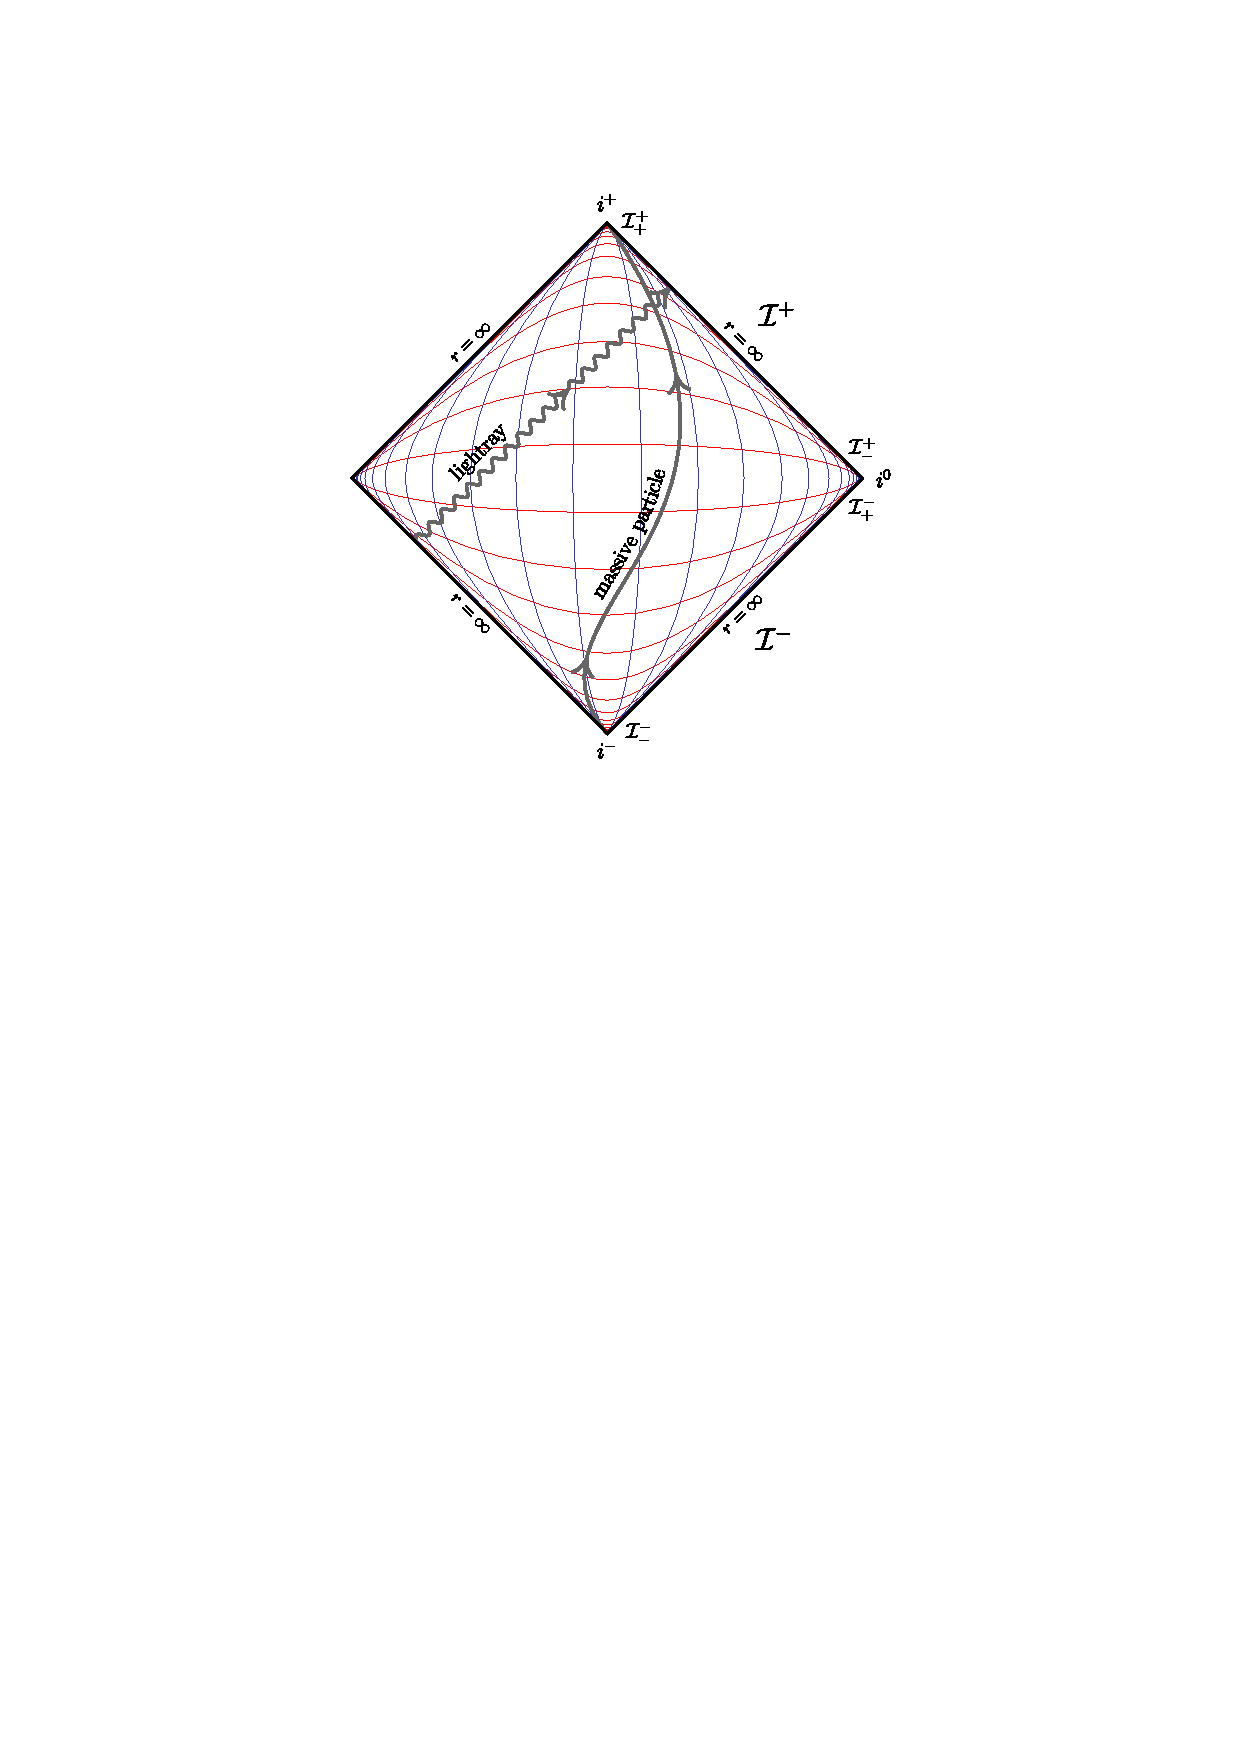
\includegraphics[width=0.618\linewidth]{figs/cover.pdf}
	\caption{Minkowski时空彭罗斯图的另一种形式}
\end{figure}

注意前面的几个Penrose图都特别对$i^+,\mathcal{I}_+^+;i^-,\mathcal{I}_-^-$以及$i^0,\mathcal{I}_+^-,\mathcal{I}_-^+$后面我们将会看到,场在这几个点上其实是多值的,或者说极限与趋近方向有关,所以必须进行区分,这几个点并不是一个点,即使是极限的意义下也不是!

在我们考虑的散射过程中,有质量粒子总是从$i^-$出发,通过类时测地线最终抵达$i^+$,而无质量粒子总是从$\mathcal{I}_-$出发走$45^\circ$斜线到达$\mathcal{I}_+$。


\section{Celestial Sphere}
\begin{figure}[htbp]
	\centering
	\tikzset{every picture/.style={line width=0.75pt}} %set default line width to 0.75pt        
	
	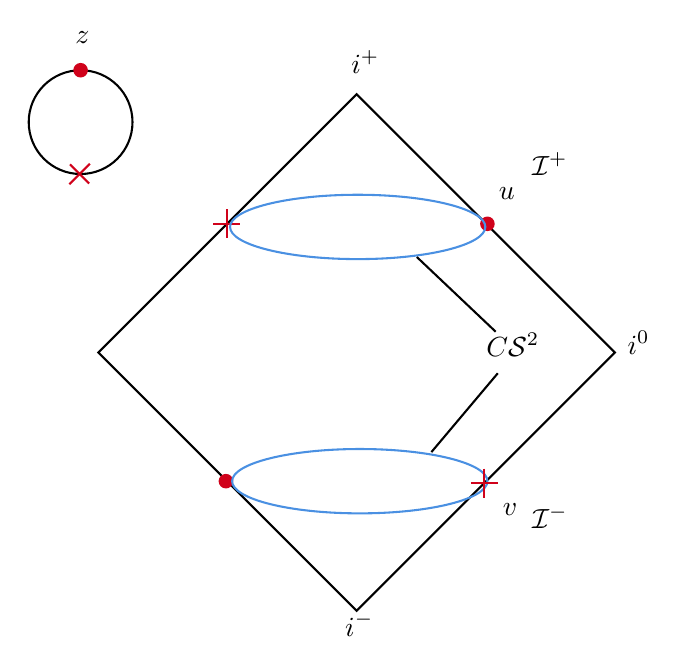
\begin{tikzpicture}[x=0.75pt,y=0.75pt,yscale=-1,xscale=1]
		%uncomment if require: \path (0,609); %set diagram left start at 0, and has height of 609
		
		%Shape: Square [id:dp4061795534153141] 
		\draw   (281,97.55) -- (405.45,222) -- (281,346.45) -- (156.55,222) -- cycle ;
		%Shape: Circle [id:dp08927835248745741] 
		\draw   (123,111) .. controls (123,97.19) and (134.19,86) .. (148,86) .. controls (161.81,86) and (173,97.19) .. (173,111) .. controls (173,124.81) and (161.81,136) .. (148,136) .. controls (134.19,136) and (123,124.81) .. (123,111) -- cycle ;
		\draw  [color={rgb, 255:red, 208; green, 2; blue, 27 }  ,draw opacity=1 ] (212,160) -- (225,160)(218.5,153) -- (218.5,167) ;
		\draw  [color={rgb, 255:red, 208; green, 2; blue, 27 }  ,draw opacity=1 ] (142.9,131.4) -- (152.1,140.6)(152.45,131.05) -- (142.55,140.95) ;
		%Shape: Circle [id:dp8549954932536064] 
		\draw  [color={rgb, 255:red, 208; green, 2; blue, 27 }  ,draw opacity=1 ][fill={rgb, 255:red, 208; green, 2; blue, 27 }  ,fill opacity=1 ] (145,86) .. controls (145,84.34) and (146.34,83) .. (148,83) .. controls (149.66,83) and (151,84.34) .. (151,86) .. controls (151,87.66) and (149.66,89) .. (148,89) .. controls (146.34,89) and (145,87.66) .. (145,86) -- cycle ;
		%Shape: Circle [id:dp26121264153734547] 
		\draw  [color={rgb, 255:red, 208; green, 2; blue, 27 }  ,draw opacity=1 ][fill={rgb, 255:red, 208; green, 2; blue, 27 }  ,fill opacity=1 ] (341,160) .. controls (341,158.34) and (342.34,157) .. (344,157) .. controls (345.66,157) and (347,158.34) .. (347,160) .. controls (347,161.66) and (345.66,163) .. (344,163) .. controls (342.34,163) and (341,161.66) .. (341,160) -- cycle ;
		%Shape: Ellipse [id:dp2797557616828865] 
		\draw  [color={rgb, 255:red, 74; green, 144; blue, 226 }  ,draw opacity=1 ] (220,161.5) .. controls (220,152.94) and (247.53,146) .. (281.5,146) .. controls (315.47,146) and (343,152.94) .. (343,161.5) .. controls (343,170.06) and (315.47,177) .. (281.5,177) .. controls (247.53,177) and (220,170.06) .. (220,161.5) -- cycle ;
		%Shape: Circle [id:dp422435135864375] 
		\draw  [color={rgb, 255:red, 208; green, 2; blue, 27 }  ,draw opacity=1 ][fill={rgb, 255:red, 208; green, 2; blue, 27 }  ,fill opacity=1 ] (215,284) .. controls (215,282.34) and (216.34,281) .. (218,281) .. controls (219.66,281) and (221,282.34) .. (221,284) .. controls (221,285.66) and (219.66,287) .. (218,287) .. controls (216.34,287) and (215,285.66) .. (215,284) -- cycle ;
		%Shape: Ellipse [id:dp2997647396682279] 
		\draw  [color={rgb, 255:red, 74; green, 144; blue, 226 }  ,draw opacity=1 ] (221,284) .. controls (221,275.44) and (248.53,268.5) .. (282.5,268.5) .. controls (316.47,268.5) and (344,275.44) .. (344,284) .. controls (344,292.56) and (316.47,299.5) .. (282.5,299.5) .. controls (248.53,299.5) and (221,292.56) .. (221,284) -- cycle ;
		\draw  [color={rgb, 255:red, 208; green, 2; blue, 27 }  ,draw opacity=1 ] (336,285) -- (349,285)(342.5,278) -- (342.5,292) ;
		%Straight Lines [id:da40913177395617817] 
		\draw    (310,176) -- (348,212) ;
		%Straight Lines [id:da5756898592429918] 
		\draw    (349,232) -- (317,270) ;
		
		% Text Node
		\draw (144,66) node [anchor=north west][inner sep=0.75pt]   [align=left] {$\displaystyle z$};
		% Text Node
		\draw (348,141) node [anchor=north west][inner sep=0.75pt]   [align=left] {$\displaystyle u$};
		% Text Node
		\draw[yshift=1em] (350,280) node [anchor=north west][inner sep=0.75pt]   [align=left] {$\displaystyle v$};
		% Text Node
		\draw (342,211) node [anchor=north west][inner sep=0.75pt]   [align=left] {$\displaystyle C\mathcal{S}^{2}$};
		% Text Node
		\draw (274,346) node [anchor=north west][inner sep=0.75pt]   [align=left] {$\displaystyle i^{-}$};
		% Text Node
		\draw (277,75) node [anchor=north west][inner sep=0.75pt]   [align=left] {$\displaystyle i^{+}$};
		% Text Node
		\draw (364,124) node [anchor=north west][inner sep=0.75pt]   [align=left] {$\displaystyle \mathcal{I}^{+}$};
		% Text Node
		\draw (364,294) node [anchor=north west][inner sep=0.75pt]   [align=left] {$\displaystyle \mathcal{I}^{-}$};
		% Text Node
		\draw (410,210) node [anchor=north west][inner sep=0.75pt]   [align=left] {$\displaystyle i^{0}$};
	\end{tikzpicture}
	\caption{Bondi坐标与天球}
	\label{fig:4}
\end{figure}
如图\ref{fig:4}所示,$\mathcal{I}^{\pm}$上的每一个点代表一个球面\sn{在这个图上是左右两边各一个点组成的对径点连成的圆周表示一个球面},我们称之为\text{天球}$C\mathcal{S}^2$,在SR的语境下,天球一般指观察者所看到的无限远区域,所以特指$\mathcal{I}^-$上的天球。

在类光无穷远处可以选取Bondi坐标来参数化天球,在$\mathcal{I}^+$上我们选取$(u,r,z,\bar z)$,其中$r\to \infty$,$(z,\bar z)$是球极投影到复平面来表示天球的角向坐标,这套坐标与$\{x^\mu\}$之间的关系为:
\begin{equation}
	x^\mu=\left(u+r,r\frac{z+\bar z}{1+z\bar z},ir\frac{\bar z-z}{1+z\bar z},r\frac{1-z\bar z}{1+z\bar z}\right)		
\end{equation}

在$\mathcal{I}^-$上我们选取$(v,r,z,\bar z)$,其中$r\to \infty$,注意现在角向坐标和$\mathcal{I}^+$上的选取是对径认同的关系,也就是说$z\mapsto-\frac{1}{\bar z}$:
\begin{equation}
	x^\mu=\left(v-r,-r\frac{z+\bar z}{1+z\bar z},-ir\frac{\bar z-z}{1+z\bar z},-r\frac{1-z\bar z}{1+z\bar z}\right)		
\end{equation}
从上面的式子也可看出$\mathcal{I}^\pm$上两套坐标空间部分的关系的确为空间反演,在图\ref{fig:4}中我们也通过{\color{red}$\bullet$}和{\color{red}$\times$}标记出来了。
\begin{figure}[htbp]
	\centering
	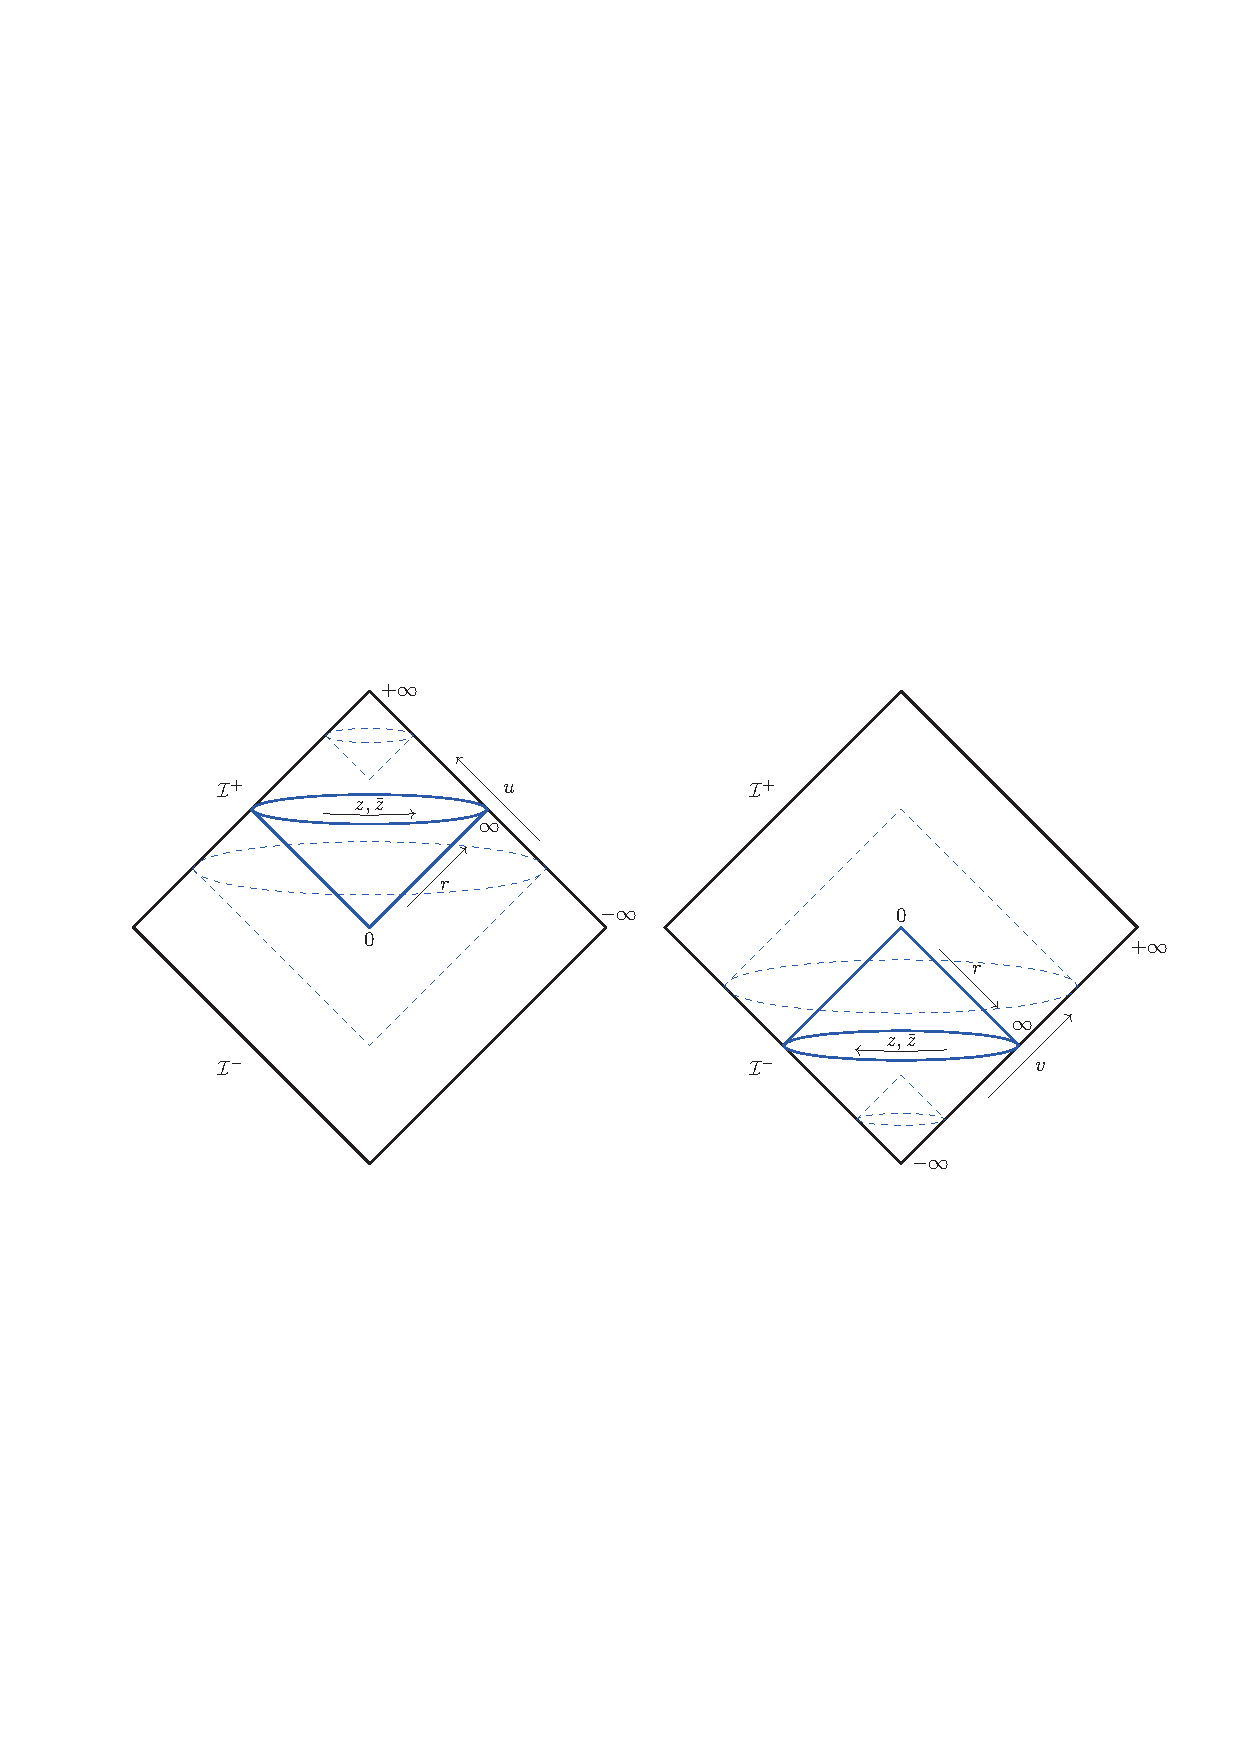
\includegraphics[width=\linewidth]{figs/fig1.pdf}
	\caption{Bondi坐标}
\end{figure}

现在考虑Lorentz变换对天球的作用,也就是要考虑Lorentz变换下Bondi坐标在$r\to\infty$怎么变。我们以$\mathcal{I}^+$上的天球为例,首先考虑$r$的变化。思路就是根据$r=\sqrt{x^ix_i}$,$x^\mu\mapsto{\Lambda^\mu}_{\nu}x^\nu$以及$SO(3,1)^\uparrow\cong SL(2,\mathbb{C})/\mathbb{Z}_2$导致的\ref{eq:8.1}进行计算,并取$r\to\infty$的极限,经过冗长的计算后得到\sn{本节的详细计算参考\cite{Oblak:2015qia}}:
\begin{equation}
	r'=r\cdot\frac{|az+b|^2+|cz+d|^2}{1+z\bar z}+\mathcal{O}(1)\equiv r\cdot F(z,\bar z)+\mathcal{O}(1)
\end{equation}
所以Lorentz变换下确实会把$r=\infty\mapsto r=\infty$。$u$的变换计算相对简单,注意到
\[t^2-r^2=u^2+2ur\]
式子左边是个Lorentz不变量,现在考虑的是某个固定$u$时的天球变换,所以$r\to\infty$后说明$2ur$是个Lorentz标量,代入$r$变换关系得到:
\begin{equation}
	u'=\frac{u}{F(z,\bar z)}+\mathcal{O}\left(\frac{1}{r}\right)
\end{equation}
注意,这里说明在一般的Lorentz变换后天球并非还是天球,因为$u$的变换依赖于角向坐标。如果现在只关心天球的角向坐标怎么变,不关心变换后每个点是属于哪一“时刻”的天球,计算后发现:
\begin{equation}
	z'=\frac{az+b}{cz+d}+\mathcal{O}\left(\frac{1}{r}\right)
\end{equation}
也就是说天球角向的变换就是$C\mathcal{S}^2$上的全局共形变换!但是写出这个形式我们利用了\ref{eq:8.1},这也就是前面为何要取$\tau_1=-\sigma_1$原因,本质上就是为了让这列公式形式更加漂亮,选取$\sigma_1$也不影响变换还是一个全局共形变换。天球在Lorentz变换下的变换可以用下图总结\sn{不少精美的插图都是直接取自\cite{Strominger:2017zoo}}:
\begin{figure}[htbp]
	\centering
	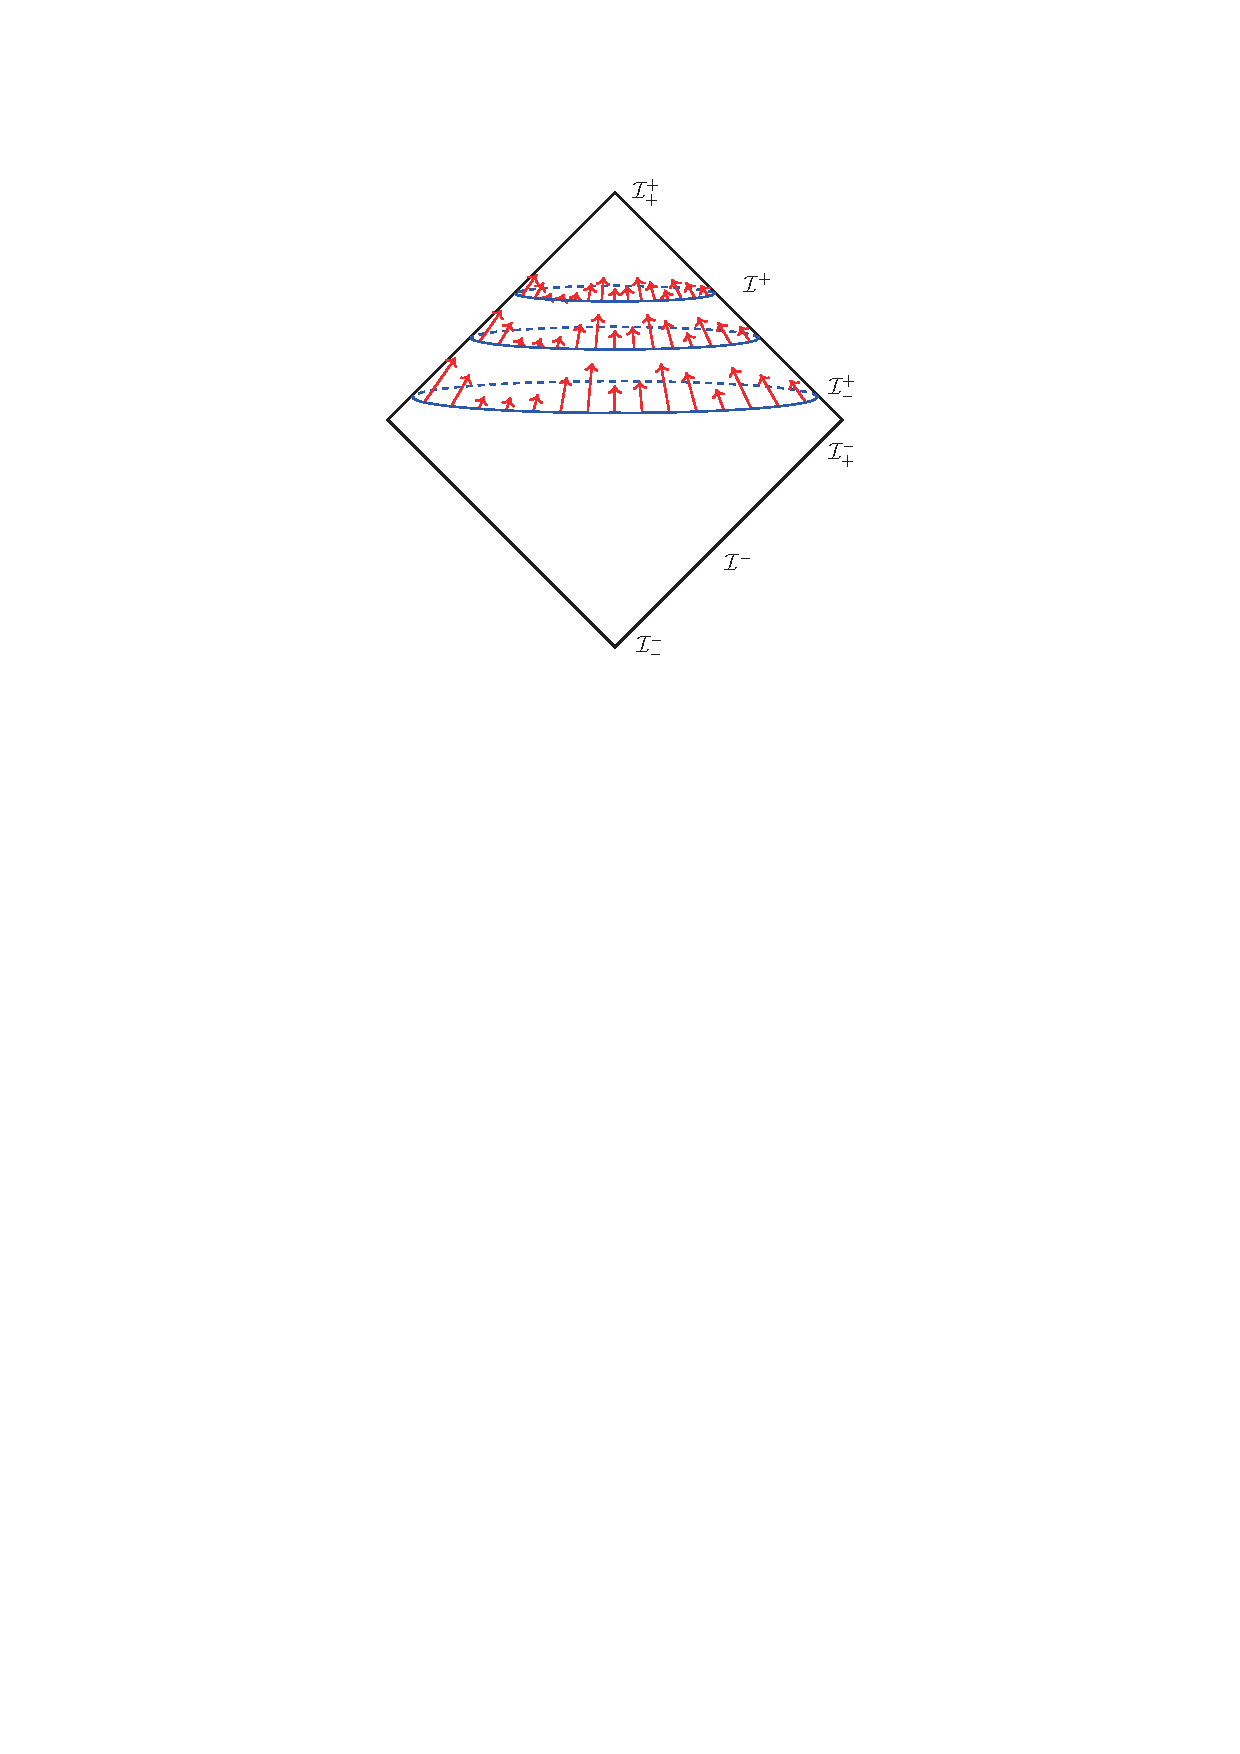
\includegraphics{figs/fig2.pdf}
	\caption{天球上的Lorentz变换}
\end{figure}

\section{Asymptotic flat spacetime: basic concepts}
所谓渐近平直时空简单点说就是在共形无限远处与Minkowski时空一致,渐近效应足够小允许存在引力波等解,但又要足够大能够排除无穷大能量这些非物理解。这一要求实际上可以用严格的与坐标无关的流形语言来描述\cite{lcb2}。这里考虑使用某一特定坐标系——Bondi坐标——的语言来进行阐述\cite{Compere:2019qed,Strominger:2017zoo},由于$\mathcal{I}^\pm$的处理方法类似,所以重点考虑于$\mathcal{I}^+$。

由于广义相对论是一个与坐标无关的理论,即理论本身具有微分同胚不变性,这是理论本身的冗余自由度,我们这里实际上是在对理论选取一个特定规范后进行描述。Bondi规范是最早也最自然的提法,当然也有其它规范选取\cite{Campiglia:2015kxa,Campiglia:2015lxa}。对于某个固定的$u(x^\mu)$,在时空上决定了一个超曲面,其上法矢为$n^\mu=g^{\mu\nu}\partial_\nu u$,第一个规范条件是要求这个超曲面类光\sn{关于超曲面的严格定义以及相关概念可参考\cite{lcb}},也就是说$n^\mu n_\mu=0\Rightarrow g^{uu}=0$;再定义$x^A,A=\{1,2\}$为角向坐标,与超曲面法矢相正交,即$\nabla_n x^A=n^\mu\partial_\mu x^A=0\Rightarrow g^{uA}=0$;最后一个要求是$r$取为\textbf{luminosity distance},这要求$\partial_r \det (g_{AB}/r^2)=0$。则$x^\mu=(u,r,x^A)$构成Bondi规范,上面的条件也等价于:
\begin{equation}
	g_{rr}=g_{rA}=0,\quad \partial_r\det\frac{g_{AB}}{r^2}=0
\end{equation}
在这个规范下,最一般的度规可以写作:\sn{后面若无特殊说明,对角向指标$A,B$求和}
\begin{equation}
	ds^2=g_{uu}du^2+2g_{ur}dudr+2g_{uA}dudx^A+g_{AB}dx^Adx^B
\end{equation}
对于Minkowski时空,Bondi guage就是选取retarded coordinate,$u=t-r$,度规形式为:
\begin{equation}
	ds^2=-du^2-2dudr+r^2\gamma_{AB}dx^Adx^B
\end{equation}
渐近平直即要求$r\to\infty$时,时空度规与上面一致。Bondi等人计算后对渐近平直时空的度规在$r\to\infty$的渐近行为给予了如下限制\cite{Bondi:1962px,Sachs:1962wk}:
\begin{equation}\label{eq:17.4}
	\begin{aligned}
		ds^2=&-du^2-2dudr+r^2\gamma_{AB}dx^Adx^B\\
		&+\frac{2m_B}{r}du^2+rC_{AB}dx^Adx^B+D^B C_{AB}dudx^A\\
		&+\frac{1}{16r^2}C_{AB}C^{AB}dudr+\frac{1}{r}\left[\frac{4}{3}\left(N_A+u\partial_Am_B\right)-\frac{1}{8}\partial_A\left(C_{BC}C^{BC}\right)\right]dudx^A\\
		&+\frac{1}{4}\gamma_{AB}C_{CD}C^{CD}dx^Adx^B+\cdots
	\end{aligned}
\end{equation}
其中$\gamma^{AB}C_{AB}=0,C_{AB}=C_{BA}$,角向指标使用$\gamma^{AB}$进行升降,而$D^A$是与单位球面上度规$\gamma^{AB}$适配的协变导数\footnote{对于任何一个流形,给定度规后都唯一存在一个无挠的联络$\nabla$使得$\nabla_X g=0,\forall X\in\mathscr{X}(\mathcal{M})$,称为Levi-Civita联络,对应的Clifford符号$\nabla_{e_\mu}e_\nu=\Gamma_{\mu\nu}^{\lambda}e_\lambda$由下式给出:
\[\Gamma^\lambda_{\mu\nu}=\frac{1}{2}g^{\lambda\sigma}\left(\partial_\mu g_{\nu\sigma}+\partial_\nu g_{\mu\sigma}-\partial_\sigma g_{\mu\nu}\right)\]这里$\Gamma^{z}_{zz}=-\frac{2\bar z}{1+z\bar z}={\Gamma^{\bar z}_{\bar z\bar z}}^*$,其它都是0。}。这里特别注意$u,r$并不是Minkowski中的retarded coordinates!只是在$r\to\infty$时$u\approx \tilde t-\tilde r$\sn{这里的$\tilde t,\tilde r$是指Minkowski时空中的通常四维坐标,也就是使得度规为$\eta_{\mu\nu}$的坐标}。同时还要求物质能动张量满足:
\begin{align*}
	T^M_{uu}\sim\mathcal{O}(r^{-2}),& &T^M_{ur}\sim\mathcal{O}(r^{-4}),&&T^M_{rr}\sim\mathcal{O}(r^{-4})\\
	T^M_{uA}\sim\mathcal{O}(r^{-2}),&&T^M_{rA}\sim\mathcal{O}(r^{-3}),&&T^M_{AB}\sim\mathcal{O}(r^{-1})
\end{align*}
而且由于是在$\mathcal{I}^+$上考虑问题,所以这些能动张量都来源于无质量粒子。

\ref{eq:17.4}引进的这些参数都是有具体的物理意义的:
\begin{itemize}
	\item[$\bullet$]$m_B$:\textbf{Bondi mass aspect},物理意义是在$\mathcal{I}^+$的$u$处天球上观察得到的时空的能量角密度分布。\textbf{Bondi mass}可以通过积分$M(u)=\oint_{\mathcal{S}^2_\infty}\mathrm{d}^2\Omega m_B(u,x^A)$给出,$u\to-\infty$时,Bondi mass等于ADM能量。
	\item[$\bullet$]$C_{AB}$:这个量根据无迹对称约束,会给出两种极化模式(或者说引力子的两个螺旋度取值),它完全确定了$\mathcal{I}^+$上的引力波辐射,根据他可以定义\textbf{Bondi news tensor} $N_{AB}=\partial_u C_{AB}$,这个量可以和电磁Fraday张量$F_{uz}=\partial_u A_z$\sn{后面章节将会看到为何是这个形式}类比,它的平方正比于$\mathcal{I}^+$上的能流。
	\item[$\bullet$]$N_A$:\textbf{angular momentum aspect},这是相对于$r=0$这一点的角动量角密度分布,对他在$\mathcal{S}^2_\infty$上积分得到在$\mathcal{I}^+$的$u$处天球上观察得到的时空的总角动量。
\end{itemize}

现在我们选取角向坐标为$x^A=(z,\bar z)$来简化讨论,更一般的讨论见\cite{Compere:2019qed}。这导致$\gamma_{AB}$对角项为0,由$C_{AB}$的无迹对称性质有$C_{zz}C^{zz}=C_{\bar z\bar z}C^{\bar z\bar z}$,实际上这个条件可以强化为$(C_{zz})^*=C_{\bar z\bar z}$。在这样的角向坐标选取下,\ref{eq:17.4}简化为\sn{注意到这里忽略了$r^{-2}dudr$贡献,而且相比于$r^2dzd\bar z$忽略了\ref{eq:17.4}最后一项$\mathcal{O}(1)$的贡献}:
\begin{equation}\label{eq:17.5}
	\begin{aligned}
		ds^2=&-du^2-2dudr+2r^2\gamma_{z\bar z}dzd{\bar z}\\
		&+\frac{2m_B}{r}du^2+rC_{zz}dz^2+rC_{\bar z\bar z}d{\bar z}^2+D^z C_{zz}dudz+D^{\bar z}C_{\bar z\bar z}dud\bar z\\
		&+\frac{1}{r}\left[\frac{4}{3}\left(N_z+u\partial_zm_B\right)-\frac{1}{4}\partial_z\left(C_{zz}C^{zz}\right)\right]dudz+c.c.+\cdots
	\end{aligned}
\end{equation}
其中$C_zz,N_z,m_B$按照\ref{eq:17.4}类似定义,而且只与$(u,z,\bar z)$有关,与$r$无关。所以渐近平直时空的度规渐近式(在Bondi gauge下)可以概括为:
\begin{align*}
	&g_{uu}=-1+\mathcal{O}(r^{-1}),&&g_{ur}=-1+\mathcal{O}(r^{-2}),&&g_{uz}=\mathcal{O}(1)\\
	&g_{zz}=\mathcal{O}(1),&&g_{z\bar z}=r^2\gamma_{z\bar z}+\mathcal{O}(1),&&g_{rr}=g_{rz}=0
\end{align*}
在不少文献中\cite{Pasterski:2021rjz,Kapec:2014opa,Raclariu:2021zjz}也经常见到\ref{eq:17.5}的另一种等价写法\sn{等价性并不显然,实际上,说他们等价,并不是说可以直接通过\ref{eq:17.5}得到\ref{eq:17.6},而是\ref{eq:17.6}形势下参量由场方程诱导的$N_z$的约束条件的形式会与\ref{eq:17.5}中的不同,他们的等价性隐藏在约束条件之中了。}:
\begin{equation}\label{eq:17.6}
	\begin{aligned}
		ds^2=&-du^2-2dudr+2r^2\gamma_{z\bar z}dzd{\bar z}\\
		&+\frac{2m_B}{r}du^2+rC_{zz}dz^2+rC_{\bar z\bar z}d{\bar z}^2+2g_{uz}dudz+2g_{u\bar z}dud\bar z+\cdots
	\end{aligned}
\end{equation}
其中:
\begin{equation}
	g_{uz}=\frac{1}{2}D^zC_{zz}+\frac{1}{6r}C_{zz}D_zC^{zz}+\frac{2}{3r}N_z+\mathcal{O}(r^{-2})
\end{equation}
不过这些对度规的限制都只是纯粹的几何意义上的,度规还必须是爱因斯坦场方程的解\sn{不少文献直接选取单位为$c=\hbar=8\pi G=1$,但是这样做实际上消去了所有量纲,无法再使用量纲分析这一工具\cite{Tong}。}:
\begin{equation}
	R_{\mu\nu}-\frac{1}{2}g_{\mu\nu}R=8\pi G T^M_{\mu\nu}
\end{equation}
\begin{remark}
	这里我们讨论一下前面对度规的约束为何是纯几何的,以\ref{eq:17.5}为例,我们计算$dudz$这一项的系数,我们先暂且设为$U_z$,根据Weyl张量(在Weyl变换下不变)的定义:
	\begin{equation}
		C_{\mu\nu\rho\sigma}=R_{\mu\nu\rho\sigma}+\frac{1}{2}\left(g_{\nu\rho}R_{\sigma\mu}+g_{\mu\sigma}R_{\rho\nu}-g_{\nu\sigma}R_{\rho\mu}-g_{\mu\rho}R_{\sigma\nu}\right)+\frac{1}{6}R\left(g_{\mu\rho}g_{\sigma\nu}-g_{\mu\sigma}g_{\rho\nu}\right)
	\end{equation}
	我们感兴趣的是下面两个分量:
	\begin{equation}
		C_{rzzrz}=R_{rzrz}-\frac{1}{2}g_{zz}R_{rr},\quad C_{rurz}=R_{rurz}+\frac{1}{2}(g_{ur}R_{rz}-g_{uz}R_{rr})
	\end{equation}
	代入$ds^2$一通计算猛如虎:
	\begin{equation}
		C_{rzzrz}=\mathcal{O}(r^{-3}),\quad C_{rurz}=-\frac{1}{4r^2}\left(U_z-D^z C_{zz}\right)+\mathcal{O}(r^{-3})
	\end{equation}
	显然,为了满足渐近平直性,要求$U_z=D^zC_{zz}$,推导过程中我们完全没有使用场方程。
\end{remark}
使用\ref{eq:17.6}的约定,利用场方程代入度规进行计算,逐项比较得到三个量满足的约束条件为:
\begin{equation}
	\begin{aligned}
		\partial_u m_B=&\frac{1}{4}D_z^2N^{zz}+\frac{1}{4}D_{\bar z}^2N^{\bar z\bar z}-\frac{1}{2}T^M_{uu}-\frac{1}{4}N_{zz}N^{zz}\\
		\partial_u N_z=&-\frac{1}{4}\left(D_zD_{\bar z}^2C^{\bar z\bar z}-D^3_zC^{zz}\right)-T^{M}_{uz}+\partial_z m_B+\frac{1}{16}D_z\partial_u(C_{zz}C^{zz})\\
		&-\frac{1}{4}N^{zz}D_zC_{zz}-\frac{1}{4}N_{zz}D_zC^{zz}-\frac{1}{4}D_z\left(C^{zz}N_{zz}-N^{zz}C_{zz}\right)
	\end{aligned}
\end{equation}
其中
\begin{equation}
	T_{\mu\nu}(u,z,\bar z)=8\pi G\lim_{r\to\infty}r^2 T^M_{\mu\nu}(u,z,\bar z)
\end{equation}

对$\mathcal{I}^{-}$可以类似分析,这里仅罗列结果\sn{这里$r\to\infty,v\approx t+r$,角向坐标与$\mathcal{I}^{+}$上的对径认同}:
\begin{equation}
	\begin{aligned}
		ds^2=&-dv^2+2dvdr+2r^2\gamma_{z\bar z}dzd{\bar z}\\
		&+\frac{2m^-_B}{r}dv^2+rD_{zz}dz^2+rD_{\bar z\bar z}d{\bar z}^2+2g_{vz}dvdz+2g_{v\bar z}dvd\bar z+\cdots
	\end{aligned}
\end{equation}
其中\sn{这里$D^{AB}$相当于前面的$C^{AB}$,不要与协变导数弄混!}
\begin{equation}
	g_{vz}=-\frac{1}{2}D^zD_{zz}-\frac{1}{6r}D_{zz}D_zD^{zz}-\frac{2}{3r}N^-_z+\mathcal{O}(r^{-2})
\end{equation}
类似的可以定义News tensor:
\begin{equation}
	M_{zz}\equiv \partial_v D_{zz}
\end{equation}
约束条件为:
\begin{equation}
	\begin{aligned}
		\partial_u m^-_B=&\frac{1}{4}D_z^2M^{zz}+\frac{1}{4}D_{\bar z}^2M^{\bar z\bar z}+\frac{1}{2}T^M_{vv}+\frac{1}{4}M_{zz}M^{zz}\\
		\partial_u N^-_z=&\frac{1}{4}\left(D_zD_{\bar z}^2D^{\bar z\bar z}-D^3_zD^{zz}\right)-T^{M}_{vz}-\partial_z m^-_B+\frac{1}{16}D_z\partial_v(C_{zz}C^{zz})\\
		&-\frac{1}{4}M^{zz}D_zD_{zz}-\frac{1}{4}M_{zz}D_zD^{zz}-\frac{1}{4}D_z\left(D^{zz}M_{zz}-M^{zz}D_{zz}\right)
	\end{aligned}
\end{equation}

渐近平直时空也可以从时空图上一窥其特征\cite{zhaoliu},只要是渐近平直时空,Penrose图在$\mathcal{I}^\pm$边界上都类似于Minkowski时空图的直角形状。

\section{Asymptotic flat spacetime: BMS group}
根据前一节的渐近分析,我们是在寻找满足一系列边界条件的规范变换(微分同胚),这些就是所谓的Allowed Symmetries,但是那些不改变物理,没有啥效应的对称性要剔除掉\sn{或者说我们需要它们能生成非0守恒荷},得到我们要找的\textbf{渐近对称性}
\begin{equation}
	\text{Asymptotic symmetries}=\frac{\text{Allowed symmetries}}{\text{Trivial symmetries}}
\end{equation}

按理说在无穷远处时空渐近平直,那么在无穷远处的渐近对称性应该就是Poinccre\'e群,但是由于渐近平直带来的高阶项(描述无穷远处的引力波扰动),这会导致体系的对称性远远大于Poincar\'e群。这从某种程度上也意味着,弱场、大尺度近似下广义相对论并不会退化为狭义相对论!

所谓AFS的对称变换,并不要求是等度规映射,仅仅要求保持Bondi gauge以及渐近平直性,这其实是要求下面的asymptotic invariant:
\begin{align*}
	&\mathcal{L}_\xi g_{uu}=\mathcal{O}(r^{-1}),&&\mathcal{L}_\xi g_{ur}=\mathcal{O}(r^{-2}),&&\mathcal{L}_\xi g_{uz}=\mathcal{O}(1)\\
	&\mathcal{L}_\xi g_{zz}=\mathcal{O}(1),&&\mathcal{L}_\xi g_{z\bar z}=\mathcal{O}(1),&&\mathcal{L}_\xi g_{\bar z \bar z}=\mathcal{O}(1)
\end{align*}
和gauge invariant:
\begin{equation}
	\mathcal{L}_\xi g_{zz}=\mathcal{L}_\xi g_{rz}=0
\end{equation}
计算后发现\sn{相当冗长的计算,细节请参考:\cite{Bondi:1962px,Sachs:1962wk,Barnich:2009se,Barnich:2010ojg,Barnich:2011mi,Barnich:2010eb}}这要求矢量场形式为:
\begin{equation}
	\begin{aligned}
		\xi^+=&\eqnmarkbox[red]{node1}{\left(1+\frac{u}{2r}\right)Y^{+z}\partial_z-\frac{u}{2r}D^{\bar z}D_zY^{+z}\partial_{\bar z}-\frac{1}{2}(u+r)D_zY^{+z}\partial_r+\frac{u}{2}D_zY^{+z}\partial_u+c.c.}\\
		&+\eqnmarkbox[blue]{node2}{f^+\partial_u-\frac{1}{r}\left(D^zf^+\partial_z+D^{\bar z}f^+\partial_{\bar z}\right)+D^zD_zf^+\partial_r}
	\end{aligned}
\end{equation}
\annotate[yshift=0.7em]{}{node1}{$\text{Superrotation  }\xi_Y^+$}
\annotate[yshift=-0.7em]{below,label below}{node2}{$\text{Supertranslation  }\xi_f^+$}

\noindent 其中,$f(z,\bar z)$是$C\mathcal{S}^2$上的任意函数,而$Y^{+z}$在$C\mathcal{S}^2$上全纯:\sn{就是$\mathcal{S}^2$上的共形Killing场之分量}
\begin{equation}\label{Y}
	\partial_{\bar z}Y^{+z}=0
\end{equation}

首先来看相对比较简单的supertranslation,可以验证,当$f$取为常函数,其生成$u$方向的平移,其它三个方向平移则由$Y_1^{\{0,\pm1\}}$生成\sn{这里$Y_\ell^m$指球谐函数}。所以下面这四个$f$:
\begin{equation}\label{f}
	f_0=1,\quad f_1=\frac{z+\bar z}{1+z\bar z},\quad f_2=\frac{i\left(\bar z-z\right)}{1+z\bar z},\quad f_3\frac{1-z\bar z}{1+z\bar z}
\end{equation}
所对应的生成元正好是Poincar\'e群的四个方向平移,进一步$f$扩展为任意函数,就变成了所谓“supertranslation”。在无穷小的supertranslation下$N_{zz},m_B,C_{zz}$的改变可以由下式定量刻画\sn{略去了后面应乘的无穷小参数}:
\begin{equation}
	\begin{aligned}
		&\delta_{f^+}N_{zz}=f^+\partial_u N_{zz}\\
		&\delta_{f^+} m_B=f^+\partial_u m_B+\frac{1}{4}\left[N_{zz}D_z^2f^++2D_zN^{zz}D_zf^++c.c.\right]\\
		&\delta_{f^+} C_{zz}=f^+\partial_u C_{zz}-2D_z^2f^+
	\end{aligned}
\end{equation}

Minkowski时空自然渐近平直,对应的三个参数都为0,上式中前两个为0,可以解释为换一下坐标系不会改变质量,也不会产生引力波。但是第三个式子不为0,这意味着渐近对称性在Minkowski时空中被破缺,容易验证当且仅当$f$取\ref{f}的四个值时,对应Poincar\'e群的平动,会让$\delta_{f^+} C_{zz}=0$。这种对称性的自发破缺实际上意味着经典引力中的真空不唯一,且存在Goldstone粒子\cite{Strominger:2017zoo}。

再来看superrotation,首先注意到$Y^{+z}$全纯,这意味着其在$C\mathcal{S}^2$上全局解析,否则在极点处不满足\ref{Y}。这说明$Y^{+z}$只能取为全局共形变换Mobi\"us变换形式,构成Witt代数的$\mathfrak{sl}(2,\mathbb{C})$子代数,有六个分量,通常取为:\sn{也简记为$Y^z=1,z,z^2,i,iz,iz^2$,是$\mathcal{S}^2$上global Kiling vector的基底}
\begin{align*}
	&Y^{+z}_{12}=-iz,&&Y^{+z}_{13}=\frac{1}{2}(1+z^2),&&Y^{+z}_{23}=\frac{i}{2}(1-z^2)\\
	&Y^{+z}_{03}=-z,&&Y^{+z}_{01}=\frac{1}{2}(1-z^2),&&Y^{+z}_{02}=\frac{i}{2}(1+z^2)
\end{align*}
事实上,这六个函数对应的正是$SO(3,1)^\uparrow$的六个boost和rotation!所以BMS群的superrotation对应的就是Lorentz群:
\begin{equation}
	\text{BMS}=SO(3,1)^\uparrow\ltimes\text{Supertranslation} 
\end{equation}
所以,BMS群在最初的意义上并没有superrotation,只是单纯的rotation。但是,文献\cite{Barnich:2009se,Barnich:2010ojg,Barnich:2011mi,Banks:2003vp}指出,真正的渐近对称性或许应该是下面的所谓\textbf{extended BMS group}:
\begin{equation}
	\text{extended BMS} =\text{Superrotation}\ltimes\text{Supertranslation}
\end{equation}
也就是说,那些local的解析函数$Y^{+z}$也应当是渐近对称性,这样的话,渐近对称性也变成无限维对称性,superrotation部分与天球上共形变换一一对应。

在superrotation下度规前系数的变换可以写为\sn{这里$\mathcal{L}_{Y^+}\equiv\mathbf{Y}^+\cdot \mathbf{D}+2D_zY^z$,这一点可以从把$C_{zz}$看作$(0,2)$张量场分量,然后利用\ref{lie}求李导数看出}:
\begin{equation}
	\begin{aligned}
		&\delta_{Y^+}C_{zz}=\frac{u}{2}\left(D_zY^{+z}+D_{\bar z}Y^{+\bar z} \right)\partial_u C_{zz}+\mathcal{L}_{Y^+}C_{zz}-\frac{1}{2}\left(D_zY^{+z}+D_{\bar z}Y^{+\bar z}\right)C_{zz}-uD^3_{z}Y^{+z}\\
		&\delta_{Y^+}N_{zz}\equiv\partial_u\delta_{Y^+}C_{zz}=\frac{u}{2}\left(D_zY^{+z}+D_{\bar z}Y^{+\bar z} \right)\partial_u N_{zz}+\mathcal{L}_{Y^+}N_{zz}-D^3_zY^{+z}
	\end{aligned}
\end{equation}

对于$\text{BMS}^-$,同样可以进行讨论,这里仅罗列一些公式:

\noindent Supertranslation:
\begin{equation}
	\xi_{f^-}=-f^-\partial_v-\frac{1}{r}\left(D^zf^-\partial_z+D^{\bar z}f^-\partial_{\bar z}\right)+D^zD_zf^-\partial_r
\end{equation}
\begin{equation}
	\begin{aligned}
		&\delta_{f^-}M_{zz}=f^-\partial_v M_{zz}\\
		&\delta_{f^-}D_{zz}=f^-\partial_v D_{zz}+2D_z^2f^-
	\end{aligned}
\end{equation}
Superrotation:
\begin{equation}
	\xi_{Y^-}=\left(1-\frac{v}{2r}\right)Y^{-z}\partial_z+\frac{v}{2r}D^{\bar z}D_zY^{-z}\partial_{\bar z}-\frac{1}{2}(r-v)D_zY^{-z}\partial_r+\frac{v}{2}D_zY^{-z}\partial_v+c.c.
\end{equation}
\begin{equation}
	\begin{aligned}
		&\delta_{Y^-}D_{zz}=\frac{v}{2}\left(D_zY^{-z}+D_{\bar z}Y^{-\bar z} \right)\partial_v D_{zz}+\mathcal{L}_{Y^-}D_{zz}-\frac{1}{2}\left(D_zY^{-z}+D_{\bar z}Y^{-\bar z}\right)D_{zz}+vD^3_{z}Y^{-z}\\
		&\delta_{Y^-}M_{zz}\equiv\partial_v\delta_{Y^-}D_{zz}=\frac{v}{2}\left(D_zY^{-z}+D_{\bar z}Y^{-\bar z} \right)\partial_v M_{zz}+\mathcal{L}_{Y^-}M_{zz}+D^3_zY^{-z}
	\end{aligned}
\end{equation}

文献\cite{Barnich:2010ojg,Barnich:2010eb}中详细讨论了$\mathfrak{bms}_n$及其中心扩张,BMS$_{d+2}$/CFT$_d$对应以及charge algebra。

\section{Asymptotic flat spacetime: charges}
时空连续对称性会诱导守恒荷,量子化后变成算符,是后面Ward恒等式的出发点。
\subsection{Noether theorem}
考虑下面的对称变换:\sn{场的旋量指标等等被省略了}
\[x\to x^{\prime},\quad\Phi(x)\to\Phi^{\prime}(x^{\prime})=\mathcal{F}(\Phi(x))\]
场的变换一部分是因为场是Poincar\'e群的表示,所以坐标变换导致场的变换,另一部分是场位形自己的变换\sn{这里对Noether定理的讨论基于大黄书\cite{DiFrancesco:1997nk},大黄书的方法最标准且优雅。}。现在考虑由参数$\{\omega_a\}$标记的无穷小变换:
\[
x^{\prime\mu} =x^{\mu}+\omega_{a}\frac{\delta x^{\mu}}{\delta\omega_{a}},  \quad
\Phi^{\prime}(x^{\prime})=\Phi(x)+\omega_{a}\frac{\delta\mathcal{F}}{\delta\omega_{a}}(x).
\]
下面的式子给出了变换生成元$G_a$的定义:
\begin{equation}
	\delta_\omega\Phi(x)\equiv\Phi'(x)-\Phi(x)\equiv-i\omega_aG_a\Phi(x)
\end{equation}
考虑这个对称变换下作用量的改变:
\begin{equation}
	\begin{aligned}
		\mathcal{S}^\prime& =\int\mathrm{d}^{d}x^{\prime}{\mathcal L}(\Phi^{\prime}(x^{\prime}),\partial_{\mu}^{\prime}\Phi^{\prime}(x^{\prime}))  \\
		&=\int\mathrm{d}^{d}x\left|\frac{\partial x^{\prime}}{\partial x}\right|\mathcal{L}(\mathcal{F}(\Phi(x)),(\frac{\partial x^{\nu}}{\partial x^{\prime\mu}})\partial_{\nu}\mathcal{F}(\Phi(x)))\\
		&=\int\mathrm{d}^dx\left(1+\partial_\mu(\omega_a\frac{\delta x^\mu}{\delta\omega_a})\right)\mathcal{L}\left(\Phi+\omega_a\frac{\delta\mathcal{F}}{\delta\omega_a},\left(\delta_\mu^\nu-\partial_\mu(\omega_a\frac{\delta x^\nu}{\delta\omega_a})\right)\left(\partial_\nu\Phi+\partial_\nu(\omega_a\frac{\delta\mathcal{F}}{\delta\omega_a})\right)\right)
	\end{aligned}
\end{equation}
注意到我们谈论对称性是在说作用量变分为$0$,$\omega_a$是一簇与坐标无关的参数,但我们推导过程中可以把他们看作是一簇函数,但是对称变换是指这些函数变成常函数之后要有$\delta S=0$。所以,上面的式子最后肯定正比于$\omega_a(x)$的导数,保留到一阶:
\begin{equation}\label{eq:19.2}
	\delta\mathcal{S}=-\int\mathrm{d}^{d}xj_{a}^{\mu}\partial_{\mu}\omega_{a}=\int\mathrm{d}^{d}x\partial_{\mu}j_{a}^{\mu}\omega_{a}
\end{equation}
其中:
\begin{equation}\label{eq:19.3}
	\boxed{
		j_a^\mu=\left(\frac{\partial\mathcal{L}}{\partial(\partial_\mu\Phi)}\partial_\nu\Phi-\delta_i^\mu\mathcal{L}\right)\frac{\delta x^\nu}{\delta\omega_a}-\frac{\partial\mathcal{L}}{\partial(\partial_\mu\Phi)}\frac{\delta\mathcal{F}}{\delta\omega_a}
	}
\end{equation}
利用这种比较巧妙的思想我们得到了在$\{\omega_a(x)\}$的变换下\sn{且$\{\omega_a\}$是常数的时候是对称变换}作用量的变换。现在注意到上式是在场平衡位形附近的变分,所以对于在壳的场,必然有式\ref{eq:19.2}对于任意的$\{\omega_a(x)\}$均为0,即连续对称性给出了守恒流\ref{eq:19.3}:
\begin{equation}
	\boxed{\partial_\mu j^\mu_a=0}
\end{equation}
对应的可以定义不随时间变化的守恒荷:
\begin{equation}
	Q_a=\int\mathrm{d}^{d-1}xj_a^0
\end{equation}
注意到对守恒流的定义其实可以相差一个反对称张量的偏导:
\[
	j_a^\mu\to j_a^\mu+\partial_\nu B_a^{\nu\mu},\quad\quad B_a^{\nu\mu}=-B_a^{\mu\nu}
\]
考虑时空平移对称性:
\[	
	\frac{\delta x^\mu}{\delta\omega^\nu}=\delta^\mu_\nu,\quad\frac{\delta\mathcal{F}}{\delta\Phi}=0
\]
这带来我们熟悉的能动量张量及其守恒律:
\begin{equation}
	\boxed{
		T_\mathsf{c}^{\mu\nu}=-\eta^{\mu\nu}\mathcal{L}+\frac{\partial\mathcal{L}}{\partial(\partial_\mu\Phi)}\partial^\nu\Phi ,\quad \partial_\mu T^{\mu\nu}=0
	}
\end{equation}
守恒流的定义可以差个反对称张量偏导数,所以可以将能动量张量对称化:
\begin{equation}
	T_\mathrm{B}^{\mu\nu}=T^{\mu\nu}+\partial_\rho B^{\rho\mu\nu},\quad B^{\rho\mu\nu}=-B^{\mu\rho\nu}
\end{equation}
对于一般的时空变换$x^{\prime\mu}=x^\mu+\omega^\mu(x)$,其实作用量的变换可以用能动量张量写成:\sn{这本质上就是能动张量的定义,能动张量编码理论在度规发生无穷下变换下的行为。}
\begin{equation}\label{eq:19.8}
	\begin{aligned}
	\delta\mathcal{S}&=\int d^dxT^{\mu\nu}\partial_{\mu}\omega_{\nu}\\
		&=\frac{1}{2}\int d^dxT^{\mu\nu}\underbrace{\left(\partial_{\mu}\omega_{\nu}+\partial_{\nu}\omega_{\mu}\right)}_{-\delta g_{\mu\nu}\equiv g(x)-{g^\prime}(x^\prime)}\\
		&=\left.-\frac{1}{2}\int d^dxT^{\mu\nu}\delta g_{\mu\nu}\right|_{g^{\mu\nu}=\eta^{\mu\nu}}
	\end{aligned}
\end{equation}

考虑共形变换为对称性,由于Poincar\'e变换是共形变换的一种,所以共形场论中仍有其散度为0,再考虑伸缩变换$\omega^\mu=\lambda x^\mu$,这将导致共形场论中能动张量无迹${T^\mu}_{\mu}=0$。

量子场论中考虑\textbf{不改变积分测度$\mathcal{D}\Phi$}的对称变换:
\begin{equation}
	\Phi^{\prime}(x)=\Phi(x)-i\omega_aG_a\Phi(x)
\end{equation}
与上面经典守恒流对应的是真空关联函数\sn{利用LSZ公式把外腿在壳之后就得到了散射振幅}意义下的Ward-Takahashi恒等式:\sn{这里的公式和\textit{Srednicki}书中不同,首先是因为\textit{Sredniki}书中convention是$\frac{\delta S}{\delta \varphi}\sim -\partial_\mu j^\mu$,比我们在\ref{eq:19.2}中多一个负号。其次是我们这里为了后面讨论二维CFT方便,已经将作用量做Wick转动,路径积分因子$\mathrm{e}^{iS}\mapsto\mathrm{e}^{-S}$。这两点共同导致了这一公式形式。}
\begin{equation}
	\boxed{
		\frac\partial{\partial x^\mu}\left\langle j_a^\mu(x)\Phi(x_1)\cdots\Phi(x_n)\right\rangle   
		=-i\sum_{i=1}^n\delta(x-x_i)\left<\Phi(x_1)\cdots G_a\Phi(x_i)\cdots\Phi(x_n)\right>
	}
\end{equation}
如果积分测度发生改变,就会出现量子反常\cite{Bilal:2008qx}。令$\mathcal{Y}=\Phi(x_2)\cdots\Phi(x_n)$,且$t=x_1^0$是$\mathcal{Y}$中最大的时间。对Ward-Takahashi恒等式在${t_-<t<t_+}\cup \mathbb{R}^3$内积分:
\begin{equation}
	\langle Q_a(t_+)\Phi(x_1)\mathcal{Y}\rangle-\langle Q_a(t_-)\Phi(x_1)\mathcal{Y}\rangle=-i\left\langle G_a\Phi(x_1)\mathcal{Y}\right\rangle
\end{equation}
取极限$t_-\to t_+$,由于$\mathcal{Y}$是任意的,所以:\sn{注意这里是在$j^\mu =T^{\mu\nu}\omega_\nu$的convention下,不同文献convention不同常常会差个负号。另外,不少文献中也会把$\delta\omega_a$吸收进左侧$Q$的定义中,这样右侧就直接是$\delta \Phi$了。}
\begin{equation}
	\boxed{
	[Q_a,\Phi]=-iG_a\Phi =\frac{\delta_\omega \Phi}{\delta \omega_a}}
\end{equation}
量子化后,在算符的意义下,守恒荷是对称性的生成元。\sn{你去用$\phi_a,\pi^a$之间的正则对易关系当然也能得到这一点,比如Srednicki\cite{srednicki},只是这里我们是完全用路径积分量子化的方法。}

广义相对论那边更多的使用所谓广义Noether定理,可以见\cite{Compere:2019qed}第一章的介绍。
\subsection{Komar Integral \& ADM}
广义相对论里面定义守恒荷是一件很难的事情,这里介绍比较初级的理论,利用与电磁理论的对比来定义守恒荷。

利用Killing矢量$K=K^\mu\partial_\mu$,可以得到与之对偶的1\mbox{-}form,$K=K_\mu dx^\mu$,进而可以定义二形式$F\equiv dF$
\begin{lemma}[Ricci identity]
	\begin{equation}
		2\nabla_{[\mu}\nabla_{\nu]}Z^\sigma={R^\sigma}_{\rho\mu\nu}Z^\rho-T^\rho{}_{\mu\nu}\nabla_\rho Z^\sigma 
	\end{equation}
\end{lemma}
\begin{theorem}
	上面定义的$F$所满足的方程可以写成非齐次Maxwell方程的形式:
	\begin{equation}\label{eq:19.15}
		d\star F=\star j
	\end{equation}
	其中$j$和物质场能动张量有关,真空$j=0$。
\end{theorem}
\begin{proof}
	利用Ricci恒等式,由于引力无挠:
	\[(\nabla_{\mu}\nabla_{\nu}-\nabla_{\nu}\nabla_{\mu})K^{\sigma}={R^{\sigma}}_{\rho\mu\nu}K^{\rho}\]
	缩并$\mu,\sigma$:
	\[(\nabla_\mu\nabla_\nu-\nabla_\nu\nabla_\mu)K^\mu=R_{\rho\nu}K^\rho \]
	最后利用Killing方程得到:
	\[\nabla_\mu\nabla_\nu K^\mu=R_{\rho\nu}K^\rho \]
	所以:
	\[\nabla^\mu F_{\mu\nu}=\nabla^\mu\nabla_\mu K_\nu-\nabla^\mu\nabla_\nu K_\mu=-2\nabla^\mu\nabla_\nu K_\mu=-2R_{\rho\nu}K^\rho \]
	引力场方程:
	\[R_{\mu\nu}=8\pi G\left(T_{\mu\nu}-\frac12Tg_{\mu\nu}\right)\]
	显然,我们已经将$F$满足的方程写成了\ref{eq:19.15}的坐标形式。
\end{proof}
由此可以类比电磁规范理论定义Komar荷:
\begin{equation}
	\boxed{
	Q_\text{Komar}=-\frac{1}{8\pi G}\int_{\Sigma}d\star F=-\frac{1}{8\pi G}\int_{\partial\Sigma}\star F=-\frac{1}{8\pi G}\int_{\partial\Sigma}\star dK
	}
\end{equation}
若Killing场处处类时,上面的玩意儿我们叫Komar质量(能量)$M_{\text{Komar}}$。下面简要说明一下其守恒的意义。

考虑下图所示的时空子流形:
\begin{figure}[H]
	\centering
	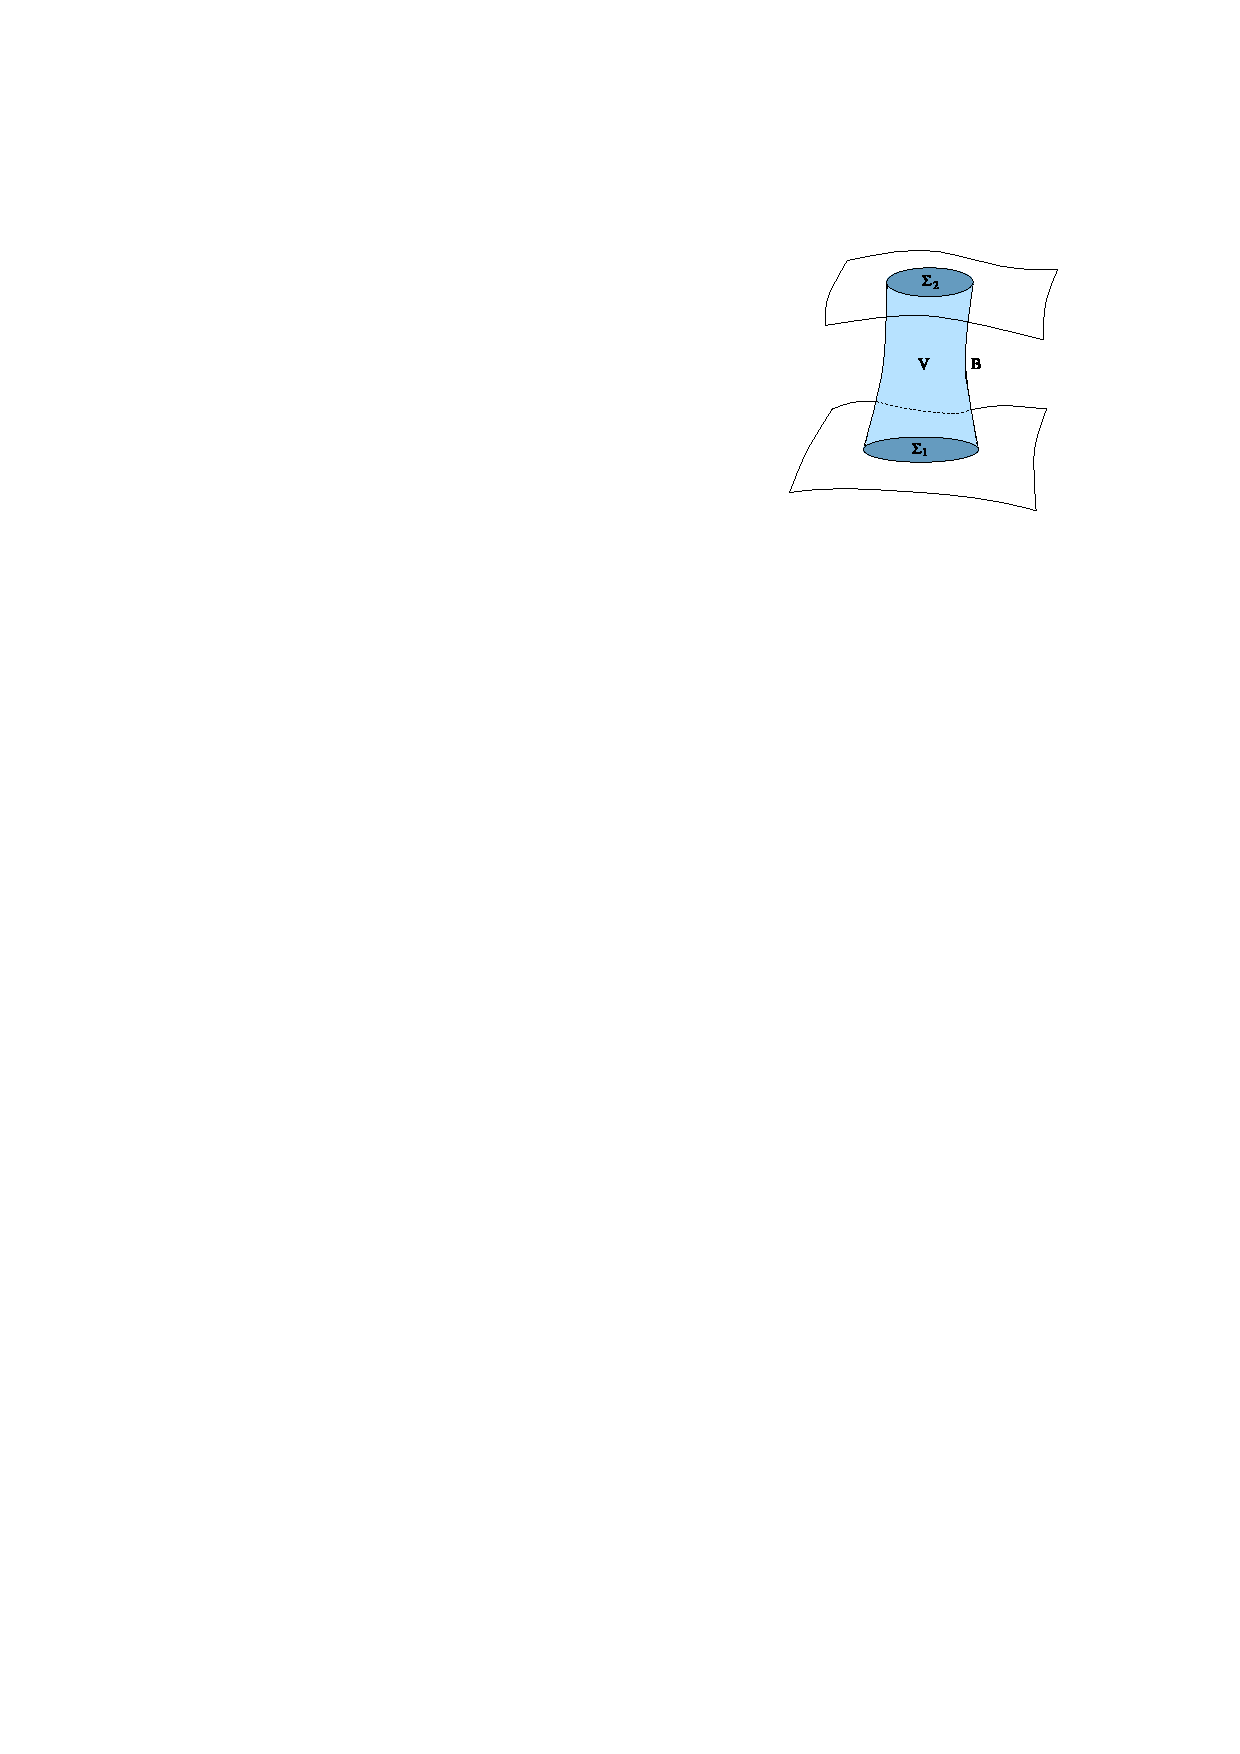
\includegraphics{figs/fig5.pdf}
\end{figure}
\noindent 其表示类空超曲面$\Sigma_1$随时间演化到$\Sigma_2$扫过的体积,其边界为:
\[\partial V=\Sigma_1\cup\Sigma_2\cup B\]
考虑$j|_B=0$的情况,这将导致下面的恒等式:
\begin{equation}
	Q_e(\Sigma_1)-Q_e(\Sigma_2)=\int_{\Sigma_1}\star J-\int_{\Sigma_2}\star J=\int_{\partial V}\star J=\int_Vd\star J=0
\end{equation}
也就是随着时间演化,某一区域的荷不变。

Komar质量依赖于类时Killing场的存在性,这对于非稳态时空是不可能的。但是对于渐近平直时空,有一种很好的定义场的总能量的方法。
\begin{definition}[ADM能量]
	假设时空度规为$g$,在某个类空超曲面$\Sigma$上诱导度规$h$,且这个类空超曲面满足存在某个坐标系$\{x^i\}$使得$r\to\infty ,h_{ij}=\delta_{ij}+\mathcal{O}(1/r)$也就是渐近平直于Euclid时空。$\mathcal{S}^2_r$是嵌在$\Sigma$中半径为$r$的球面,则ADM能量定义为:
	\begin{equation}
		\boxed{
			E_{ADM}=\dfrac{1}{16\pi G}\lim_{r\longrightarrow\infty}\int_{S_{r}^{2}}d\Omega r^{2}\hat{x}^{j}(\partial_{k}h_{jk}-\partial_{j}h_{kk})
		}
	\end{equation}
\end{definition}

前面讨论AFS时我们强调过,虽然我们在Bondi gauge下讨论问题,但是结论都是不依赖于规范的,这里ADM能量也不依赖于坐标系$\{x^i\}$的选取,虽然看起来这个定义依赖于坐标系,而且这个定义对于渐近平直的稳态时空,如果取$\Sigma$渐近正交于类时Killing场,则其与Komar质量一致。

虽然爱因斯坦场方程对于某一给定度规总能求出解,但是能动张量是否是“物理的”值得思考,对此,人们总结出了下面的三个能动张量要满足的条件。
\begin{definition}[弱能量条件]
	任意瞬时观者测得的能量密度非负,即要求:
	\begin{equation}
		T_{ab}u^au^b\geq 0,\quad\forall\text{类时矢量场 }u^a
	\end{equation}
\end{definition}

\begin{definition}[强能量条件]
	这是在证明奇性定理时提出的条件:
	\begin{equation}
		T_{ab}Z^aZ^b\geq-\frac12T\text{,}\forall\quad \text{单位类时矢量场 }Z^a
	\end{equation}
\end{definition}
\begin{definition}[主能量条件]
	本条件要求任一瞬时观者\footnote{就是$Z^a$和粒子世界线在$p$处相切,这时在观者参考系下粒子瞬时静止。这个不难理解,自由下落参考系就是通过测地线指数映射建立的,观者和粒子世界线相切说明相对静止,可做测量。}$(p,Z^a)$测得的4动量密度$W^a\equiv-{T^a}_bZ^b$是指向未来的类时或类光矢量,其物理解释是物质场的能量流动速率小于或等于光速\footnote{见经典名著\cite{Hawking:1973uf}}。
\end{definition}
这三个条件互不蕴含,不要被名字忽悠了。
\begin{theorem}[正质量定理(Schoen\&Yau)]
	若渐近平直时空没有奇异性,且物质能动张量满足主能量条件,则其ADM质量大于或等于零。当且仅当为闵氏时空时等于零。\footnote{值得注意的是,教皇Witten找到了更简单的证明\cite{Witten:1981mf,Parker:1981uy}。}
\end{theorem}

\subsection{Scattering problem}
前面使用几何学和动力学给出了$\mathcal{I}^{\pm}$上的度规约束,为了完整的解出各个参数,我们需要一些initial data\sn{关于initial data的更多讨论,以及引力理论为啥是个Cauchy问题的细节证明可见\cite{Wald:1984rg}$\S 10$}。在此,有必要先明确一下我们所考虑的一类时空,它们是所谓C-K时空\cite{ChristodoulouKlainerman+1994,PhysRevLett.67.1486},特点是在$i^{\pm}$都是真空,这给出了下面的渐近条件:
\[N_{zz}=\mathcal{O}\left(|u|^{-(1+\varepsilon)}\right),\quad\varepsilon>0\]
为了让Wyle张量在$\mathcal{I}^+_-$上归零,这要求\cite{Strominger:2013jfa,Compere:2019qed}:
\begin{equation}
	C_{zz}|_{\mathcal{I}_{-}^{+}}=-2D_{z}^{2}\bar{C}|_{\mathcal{I}_{-}^{+}}
\end{equation}
其中$C(z,\bar z)$是$\mathcal{S}^2$上的任意函数,称为Supertranslation memory field。BMS相关的文献符号不是太统一,本part后面内容的讨论我们在\ref{eq:17.5}的约定下干活,对应的我们还有如下不同于前文的符号约定:
\begin{equation}
	\begin{aligned}
	T_{uu}&\equiv\frac{1}{4}N_{zz}N^{zz}+4\pi G\lim_{r\to\infty}\left[r^2T_{uu}^M\right]	\\
	T_{uz}&\equiv8\pi G\lim_{r\rightarrow\infty}\left[r^{2}T_{uz}^{M}\right]-\frac{1}{4}\partial_{z}\left(C_{zz}N^{zz}\right)-\frac{1}{2}C_{zz}D_{z}N^{zz}
	\end{aligned}
\end{equation}
对应的约束条件变为:\sn{格外注意$N_z$的区别}
\begin{equation}
\begin{aligned}
	\partial_{u}N_{z}&=\frac{1}{4}\partial_{z}\left(D_{z}^{2}C^{zz}-D_{\bar{z}}^{2}C^{\bar{z}\bar{z}}\right)-u\partial_{u}\partial_{z}m_{B}-T_{uz}\\
	\partial_{u}m_{B}&=\frac{1}{4}\left[D_{z}^{2}N^{zz}+D_{\bar{z}}^{2}N^{\bar{z}\bar{z}}\right]-T_{uu}
\end{aligned}
\end{equation}
从约束条件以及$N^{zz}\equiv\partial_u C^{zz}$就可以看出initial data为:
\begin{equation}
	\{N_{zz}(u,z,\bar{z}),C(z,\bar{z})|_{\mathcal{I}_{-}^{+}},m^+_{B}(z,\bar{z})|_{\mathcal{I}_{-}^{+}},N^-_z|_{\mathcal{I}^+_-},\cdots\}
\end{equation}
后面的$\cdots$表示当我们考虑度规中的更高阶项时需要加入的initial data。对于$\mathcal{I}^-$类似分析可以得到initial data:
\begin{equation}
	\{M_{zz}(u,z,\bar{z}),D(z,\bar{z})|_{\mathcal{I}_{+}^{-}},m^-_{B}(z,\bar{z})|_{\mathcal{I}_{+}^{-}},N^-_z|_{\mathcal{I}^-_+},\cdots\}
\end{equation}

经典引力理论的散射问题就是在找$\mathcal{I}^+$上的Cauchy data到$\mathcal{I}^-$上的Cauchy data的映射。不过上面的initial data还无法完全使得此问题well-define,文献\cite{Strominger:2013jfa}从Lorentz和${\mathcal{CPT}}$不变性的要求出发,认为需要加入下面的对径认同假设来构成散射问题的全部:
\begin{equation}
	C(z,\bar{z})|_{\mathcal{I}_{-}^{+}}=D(z,\bar{z})|_{\mathcal{I}_{+}^{-}},\quad m^+_{B}(z,\bar{z})|_{\mathcal{I}_{-}^{+}}=m^-_{B}(z,\bar{z})|_{\mathcal{I}_{+}^{-}}.
\end{equation}
同样也要求\cite{Kapec:2014opa}:
\begin{equation}
	N^+_{z}(z,\bar{z})|_{\mathcal{I}_{-}^{+}}=N^-_{z}(z,\bar{z})|_{\mathcal{I}_{+}^{-}}
\end{equation}
这些式子也使得$BMS^+\times BMS^-$联合变换限制为一个子群,称为$\mathcal{X}$变换\cite{Kapec:2014opa},要求:
\begin{equation}
	f^+(z,\bar z)|_{\mathcal{I}^+_-}=f^-(z,\bar z)|_{\mathcal{I}^-_+},\quad Y^{+z}|_{\mathcal{I}^+_-}=Y^{-z}|_{\mathcal{I}^-_+}
\end{equation}
所以后面我们不再区分$N_z^{\pm},f^{\pm},Y^{\pm},m_B^{\pm},\{C^{zz},D^{zz}\},\{M^{zz},N^{zz}\}$,用统一的符号书写,而且在$\mathcal{I}^{\pm}_{\mp}$上对径认同。在QED中,这种对径认同也是存在的,而且可以很自然地导出。
\subsection{BMS charges}
完全可以从广相的角度去推出守恒荷,但是那太麻烦,这里直接从对径认同的条件导出守恒荷。

首先是supertranslation对应的守恒荷:\sn{这里的$d^2z\gamma_{z\bar z}$其实就是$\mathcal{S}^2$上的测度$d^2z\sqrt{\gamma}$}
\begin{equation}
	Q_{f}^{+} \equiv\frac{1}{4\pi G}\int_{{\mathcal I}_{-}^{+}}d^{2}z\gamma_{z\bar{z}}fm_{B}=
	\frac{1}{4\pi G}\int_{\mathcal{I}_{+}^{-}}d^{2}z\gamma_{z\bar{z}}fm_{B}\equiv Q_{f}^{-} 
\end{equation}
利用Stokes等式,$\partial\mathcal{I}^+=\mathcal{I}^+_-\cup\mathcal{I}^-_+$,设$m_B|_{\mathcal{I}^+_+}\to 0$并利用前面的约束方程,得到:
\begin{equation}
	\begin{gathered}
		Q_{f}^{+} =\frac1{4\pi G}\int_{\mathcal{I}^+}dud^2z\gamma_{z\bar{z}}f\left[T_{uu}-\frac14\left(D_z^2N^{zz}+D_{\bar{z}}^2N^{\bar{z}\bar{z}}\right)\right] \\
		Q_{f}^{-} =\frac1{4\pi G}\int_{\mathcal{I}^-}dvd^2z\gamma_{z\bar{z}}f\left[T_{vv}+\frac14\left(D_z^2N^{zz}+D_{\bar{z}}^2N^{\bar{z}\bar{z}}\right)\right] 
	\end{gathered}
\end{equation}
然后再是superrotation部分:
\begin{equation}
	Q_{Y}^{+}\equiv\frac{1}{8\pi G}\int_{\mathcal I_{-}^{+}}d^{2}z(Y_{\bar{z}}N_{z}+Y_{z}N_{\bar{z}})=\frac{1}{8\pi G}\int_{\mathcal I_{+}^{-}}d^{2}z(Y_{\bar{z}}N_{z}+Y_{z}N_{\bar{z}})\equiv Q_{Y}^{-}
\end{equation}
如果$Y^z$取为$\mathcal{S}^2$上共形Killing场的那六个分量,上式在说明AMD角动量和BORT center-of-mass\sn{可以见文献\cite{Chen:2014kea}中的定义}的守恒律。依旧是利用Stokes方程:\sn{与文献\cite{Pasterski:2021rjz}中的形式稍有不同,注意到$\gamma_{z\bar z}D_z Y^z=\partial_zY_{\bar z}$可以证明等价性}
\begin{equation}
	\begin{aligned}
		&Q_{Y}^{+} =Q_{H}^{+}+Q_{S}^{+},  \\
		&Q_{S}^{+} =-\frac{1}{16\pi G}\int_{\mathcal{I}^{+}}dud^{2}z[D_{z}^{3}Y^{z}uN^{z}{}_{\bar{z}}+D_{\bar{z}}^{3}Y^{\bar{z}}uN^{\bar{z}}_{z}],  \\
		&Q_{H}^{+} =\frac{1}{8\pi G}\int_{\mathcal{I}^{+}}dud^{2}z(Y_{\bar{z}}T_{uz}+Y_{z}T_{u\bar{z}}+u\partial_{z}Y_{\bar{z}}T_{uu}+u\partial_{\bar{z}}Y_{z}T_{uu}) 
	\end{aligned}
\end{equation}
我们到后面再聊它们的确是Supertranslations和Suprtrotations的生成元。